%%%%%%%%%%%%%%%%%%%%%%%%%%%%%%%%%%%%%%%%%
% Short Sectioned Assignment LaTeX Template Version 1.0 (5/5/12)
% This template has been downloaded from: http://www.LaTeXTemplates.com
% Original author:  Frits Wenneker (http://www.howtotex.com)
% License: CC BY-NC-SA 3.0 (http://creativecommons.org/licenses/by-nc-sa/3.0/)
%%%%%%%%%%%%%%%%%%%%%%%%%%%%%%%%%%%%%%%%%

%----------------------------------------------------------------------------------------
%	PACKAGES AND OTHER DOCUMENT CONFIGURATIONS
%----------------------------------------------------------------------------------------

\documentclass[paper=a4, fontsize=11pt]{scrartcl} % A4 paper and 11pt font size

% ---- Entrada y salida de texto -----

\usepackage[T1]{fontenc} % Use 8-bit encoding that has 256 glyphs
\usepackage[utf8]{inputenc}
\usepackage{hyperref}
%\usepackage{fourier} % Use the Adobe Utopia font for the document - comment this line to return to the LaTeX default

% ---- Idioma --------

\usepackage[spanish, es-tabla]{babel} % Selecciona el español para palabras introducidas automáticamente, p.ej. "septiembre" en la fecha y especifica que se use la palabra Tabla en vez de Cuadro

% ---- Otros paquetes ----

\usepackage{url} % ,href} %para incluir URLs e hipervínculos dentro del texto (aunque hay que instalar href)
\usepackage{amsmath,amsfonts,amsthm} % Math packages
%\usepackage{graphics,graphicx, floatrow} %para incluir imágenes y notas en las imágenes
\usepackage{graphics,graphicx, float} %para incluir imágenes y colocarlas

% Para hacer tablas comlejas
%\usepackage{multirow}
%\usepackage{threeparttable}

%\usepackage{sectsty} % Allows customizing section commands
%\allsectionsfont{\centering \normalfont\scshape} % Make all sections centered, the default font and small caps

\usepackage{fancyhdr} % Custom headers and footers
\pagestyle{fancyplain} % Makes all pages in the document conform to the custom headers and footers
\fancyhead{} % No page header - if you want one, create it in the same way as the footers below
\fancyfoot[L]{} % Empty left footer
\fancyfoot[C]{} % Empty center footer
\fancyfoot[R]{\thepage} % Page numbering for right footer
\renewcommand{\headrulewidth}{0pt} % Remove header underlines
\renewcommand{\footrulewidth}{0pt} % Remove footer underlines
\setlength{\headheight}{13.6pt} % Customize the height of the header

\numberwithin{equation}{section} % Number equations within sections (i.e. 1.1, 1.2, 2.1, 2.2 instead of 1, 2, 3, 4)
\numberwithin{figure}{section} % Number figures within sections (i.e. 1.1, 1.2, 2.1, 2.2 instead of 1, 2, 3, 4)
\numberwithin{table}{section} % Number tables within sections (i.e. 1.1, 1.2, 2.1, 2.2 instead of 1, 2, 3, 4)

\setlength\parindent{0pt} % Removes all indentation from paragraphs - comment this line for an assignment with lots of text

\newcommand{\horrule}[1]{\rule{\linewidth}{#1}} % Create horizontal rule command with 1 argument of height


%----------------------------------------------------------------------------------------
%	TÍTULO Y DATOS DEL ALUMNO
%----------------------------------------------------------------------------------------

\title{	
\normalfont \normalsize 
\textsc{\textbf{Ingeniería de Servidores (2016-2017)} \\ Grado en Ingeniería Informática \\ Universidad de Granada} \\ [25pt] % Your university, school and/or department name(s)
\horrule{0.5pt} \\[0.4cm] % Thin top horizontal rule
\huge Memoria Práctica 5 \\ % The assignment title
\horrule{2pt} \\[0.5cm] % Thick bottom horizontal rule
}

\author{Sergio Samaniego Martínez} % Nombre y apellidos

\date{\normalsize\today} % Incluye la fecha actual

%----------------------------------------------------------------------------------------
% DOCUMENTO
%----------------------------------------------------------------------------------------

\begin{document}

\maketitle % Muestra el Título

\newpage

\tableofcontents % para generar el índice de contenidos

\newpage

%----------------------------------------------------------------------------------------
%	Cuestión 1
%----------------------------------------------------------------------------------------

\section{Cuestión 1}

\subsection{\Large Al modificar los valores del kernel de este modo, no logramos que persistan después de reiniciar la máquina. ¿Qué archivo hay que editar para que los cambios sean permanentes?}

Como se ha dicho, con sysctl podemos realizar cambios en el kernel del sistema, pero este no será permanente.

Por ejemplo, si quiero cambiar el nombre de mi equipo, debo hacer lo siguiente:

\begin{figure}[H] %con el [H] le obligamos a situar aquí la figura
	\centering
	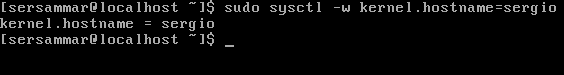
\includegraphics[scale=0.5]{imagenes/sys.png}  %el parámetro scale permite agrandar o achicar la imagen. En el nombre de archivo puede especificar directorios
	\caption{Cambio temporal del nombre de mi equipo.} \label{fig:figura1}
\end{figure}

Pero para poder hacerlo permanente, lo que debemos hacer es modificar el archivo que se encuentra en /etc/sysctl.conf  \cite{sysctl}

Para ello abrimos el archivo sysctl.conf con nuestro editor de textos.
Introducimos una línea con el  valor que queremos modificar al igual que se hizo con sysctl.

\begin{figure}[H] %con el [H] le obligamos a situar aquí la figura
	\centering
	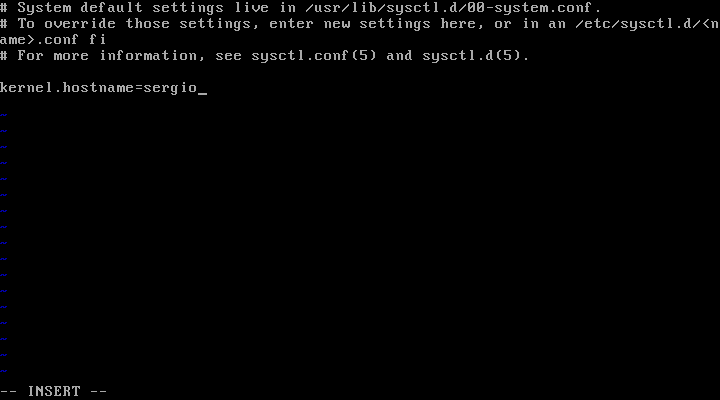
\includegraphics[scale=0.5]{imagenes/perma.png}  %el parámetro scale permite agrandar o achicar la imagen. En el nombre de archivo puede especificar directorios
	\caption{Cambio permanente del nombre de mi equipo.} \label{fig:figura2}
\end{figure}

Guardamos las modificaciones y salimos.

\begin{figure}[H] %con el [H] le obligamos a situar aquí la figura
	\centering
	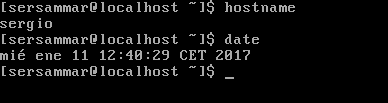
\includegraphics[scale=0.5]{imagenes/nombre-prev.png}  %el parámetro scale permite agrandar o achicar la imagen. En el nombre de archivo puede especificar directorios
	\caption{Cambio temporal del nombre de mi equipo.} \label{fig:figura3}
\end{figure}

Como vemos el nombre se ha cambiado, pero esta prueba se ha realizado antes de reiniciar el equipo. Ahora vamos a probar a reiniciarlo y ver si se han guardado los cambios.

\begin{figure}[H] %con el [H] le obligamos a situar aquí la figura
	\centering
	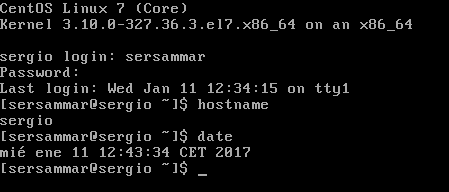
\includegraphics[scale=0.5]{imagenes/nombre-post.png}  %el parámetro scale permite agrandar o achicar la imagen. En el nombre de archivo puede especificar directorios
	\caption{Comprobación de que el cambio se ha realizado.} \label{fig:figura4}
\end{figure}


Para que los cambios se actualicen inmediatamente sin necesidad de reiniciar el sistema podemos ejecutar el comando sysctl -p 



%----------------------------------------------------------------------------------------
%	Cuestión 2
%----------------------------------------------------------------------------------------

\section{Cuestión 2}

\subsection{\Large  ¿Con qué opción se muestran todos los parámetros modificables en tiempo de ejecución? Elija dos parámetros y explique, en dos líneas, qué función tienen.}

Para ver todos los parámetros modificables con sysctl nos basta con ponerle el flag -a \cite{man-sysctl}

\begin{figure}[H] %con el [H] le obligamos a situar aquí la figura
	\centering
	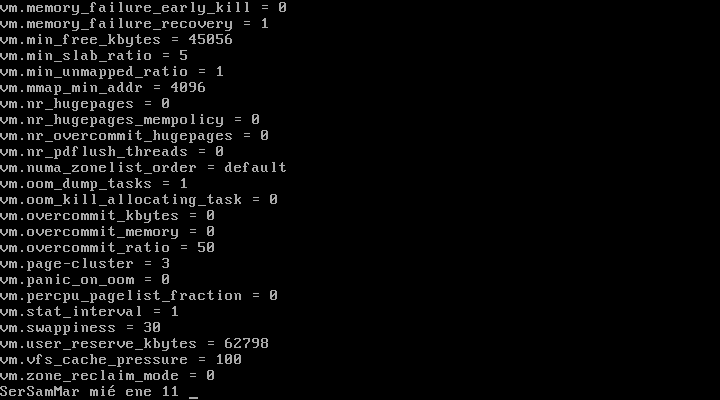
\includegraphics[scale=0.5]{imagenes/sys-a.png}  %el parámetro scale permite agrandar o achicar la imagen. En el nombre de archivo puede especificar directorios
	\caption{Algunos de los parámetros mostrados al ejecutar el comando sysctl -a } \label{fig:figura5}
\end{figure}

Dos de los parámetros de los existentes son los siguientes: 
\begin{itemize}
	\item min\_free\_kbytes: Con este valos se le obliga al sistema a que siempre deje libres tantos kBytes de memoria como se indiquen aquí. \cite{parametros}
	
	\item max\_map\_count:Este parámetro contiene el número máximo de áreas de mapas de memoria que un proceso puede tener. \cite{parametros}
\end{itemize}

%----------------------------------------------------------------------------------------


%----------------------------------------------------------------------------------------
%	Cuestión 3
%----------------------------------------------------------------------------------------
\section{Cuestión 3}

\subsection{\Large Realice una copia de seguridad del registro y restáurela,ilustre el proceso con capturas. }

Para realizar una copia de seguridad del registro debemos entrar en el editor de registro, pulsando las teclas Windows+R y escribiendo en la ventana regedit.

\begin{figure}[H] %con el [H] le obligamos a situar aquí la figura
	\centering
	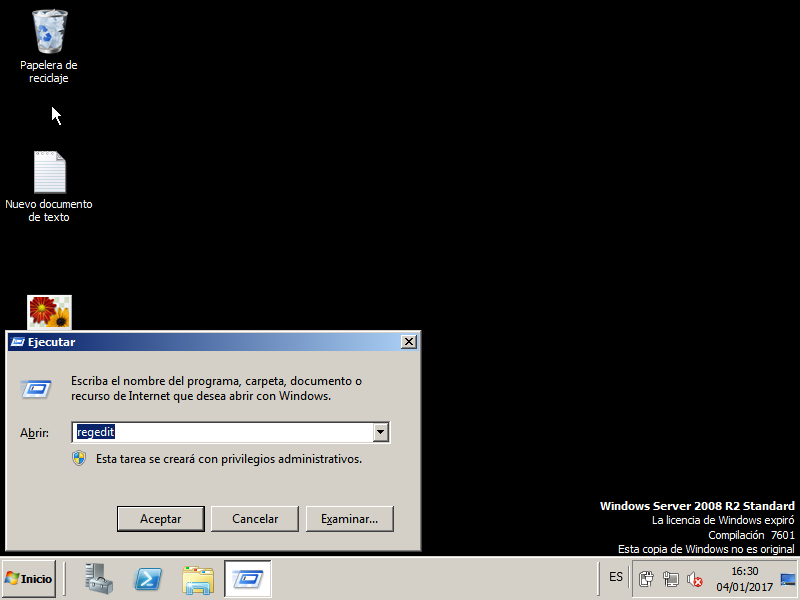
\includegraphics[scale=0.5]{imagenes/regedit.png}  %el parámetro scale permite agrandar o achicar la imagen. En el nombre de archivo puede especificar directorios
	\caption{Muestra de acceso al editor de registro desde las teclas Windows+R} \label{fig:figura6}
\end{figure}

Una vez dentro del registro, deberíamos seleccionar el registro o los registros que deseamos guardar, hacer click en Archivo->Exportar y elegir el lugar donde queramos guardar el registro.

\begin{figure}[H] %con el [H] le obligamos a situar aquí la figura
	\centering
	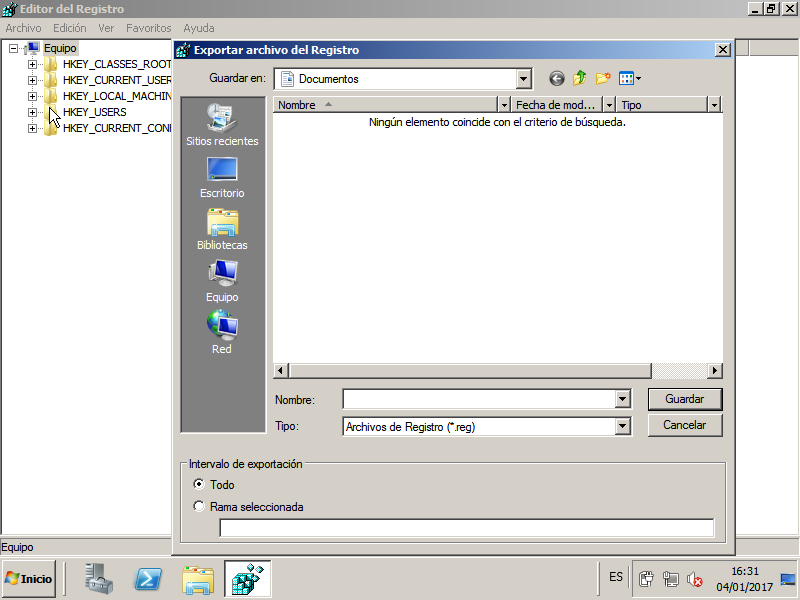
\includegraphics[scale=0.5]{imagenes/exportar.png}  %el parámetro scale permite agrandar o achicar la imagen. En el nombre de archivo puede especificar directorios
	\caption{Paso para guardar el registro en el lugar que deseamos.} \label{fig:figura7}
\end{figure}


\begin{figure}[H] %con el [H] le obligamos a situar aquí la figura
	\centering
	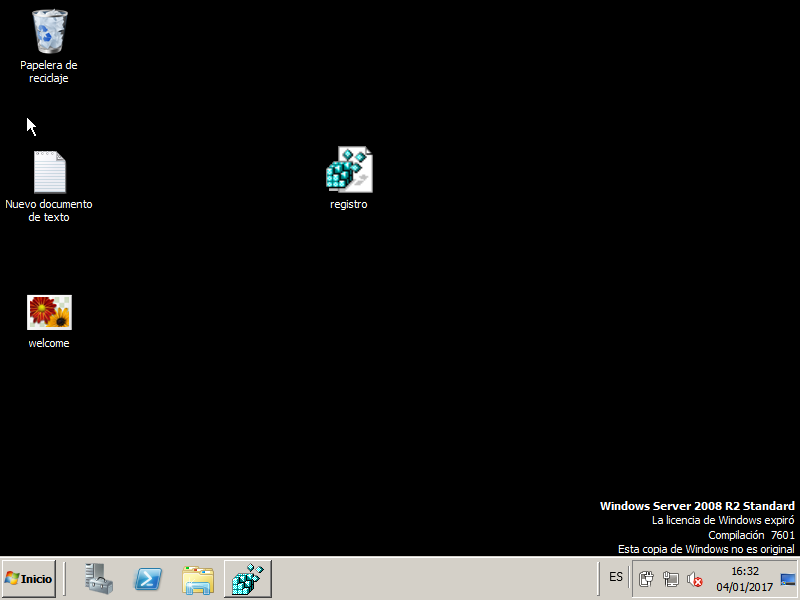
\includegraphics[scale=0.5]{imagenes/reg_guardado.png}  %el parámetro scale permite agrandar o achicar la imagen. En el nombre de archivo puede especificar directorios
	\caption{Registro guardado en el escritorio.} \label{fig:figura8}
\end{figure}

Por último, si queremos restaurar el registro podemos hacerlo de dos formas diferentes:
La primera forma es como se nos indica en la guía de la práctica, y en la página que hacemos referencia. \cite{restf8}

De esta manera, lo que debemos hacer es cuando iniciamos el sistema, y pase la pantalla de de carga de la BIOS, pulsaremos F8 para entrar en las opciones avanzadas.

Una vez dentro de las opciones avanzadas, elegiremos la opción "La última opción válida conocida(avanzada)" como mostramos en la imagen siguiente, y así podremos restablecer los valores del registro al estado que tenían la última vez que se inició el sistema correctamente.

\begin{figure}[H] %con el [H] le obligamos a situar aquí la figura
	\centering
	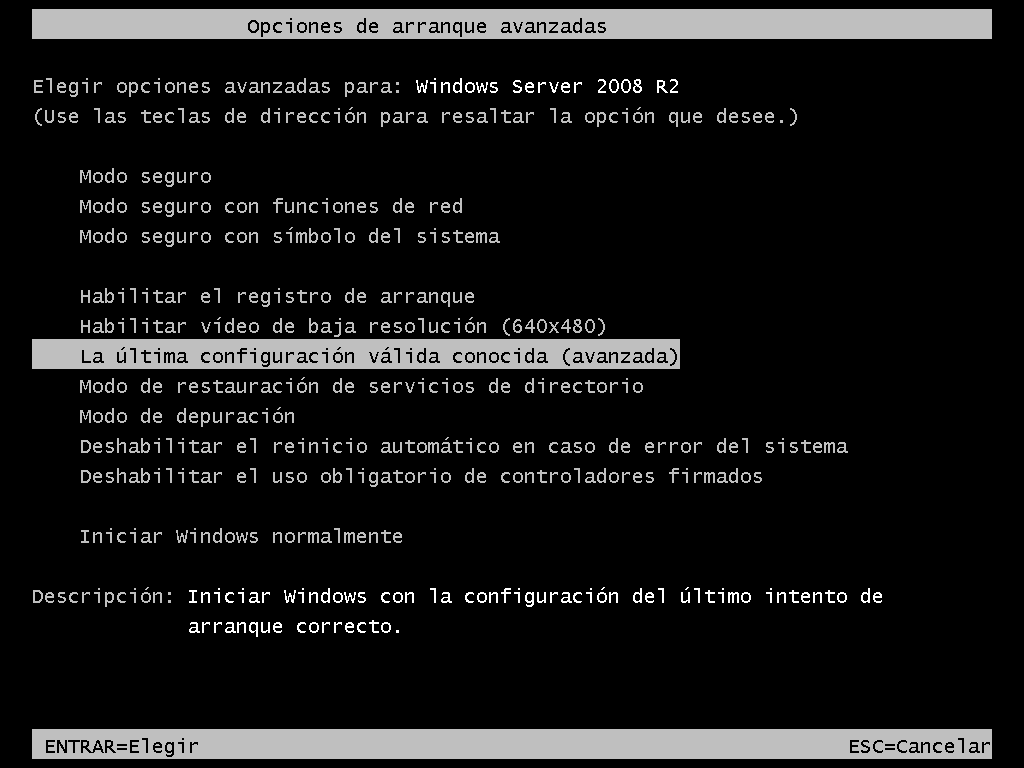
\includegraphics[scale=0.5]{imagenes/restaurar_F8.png}  %el parámetro scale permite agrandar o achicar la imagen. En el nombre de archivo puede especificar directorios
	\caption{Modo de restauración de los registros.} \label{fig:figura9}
\end{figure}


Otra opción para restaurar los registros, puede ser desde el mismo editor de registro.

Una vez dentro del editor de registro, podemos seleccionar Archivo->Importar y seleccionamos la copia de seguridad que teníamos hecha de los registros que habíamos seleccionado. \cite{rest_regedit}

\begin{figure}[H] %con el [H] le obligamos a situar aquí la figura
	\centering
	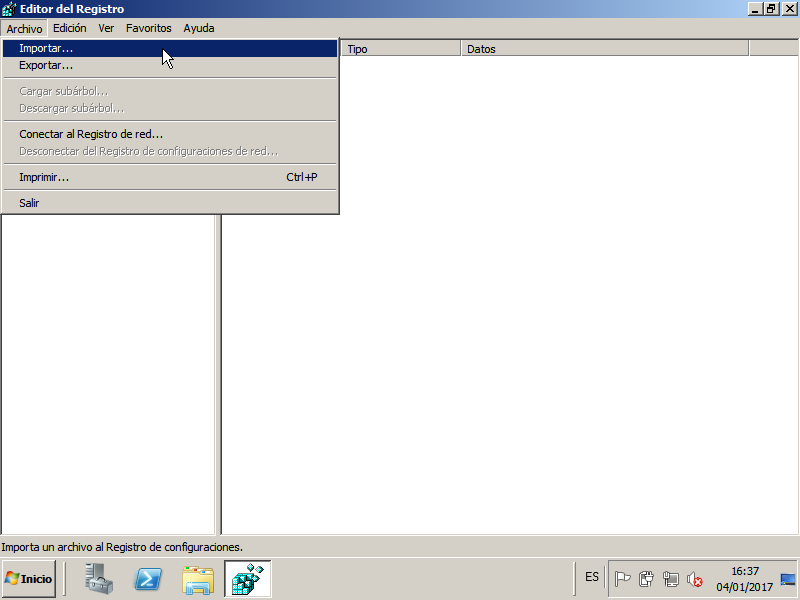
\includegraphics[scale=0.5]{imagenes/restaurar_regedit.png}  %el parámetro scale permite agrandar o achicar la imagen. En el nombre de archivo puede especificar directorios
	\caption{Modo de restauración de los registros.} \label{fig:figura10}
\end{figure}



\subsection{\Large Abra una ventana mostrando el editor del registro. }

	El editor de registro se abre como se ha comentado en el apartado anterior pulsando las teclas Windows+R y escribiendo en el cuadro de búsqueda regedit.
	
	Una vez hecho esto, entraremos en el editor de registro, que se ve como se muestra en la imagen.
	
	\begin{figure}[H] %con el [H] le obligamos a situar aquí la figura
		\centering
		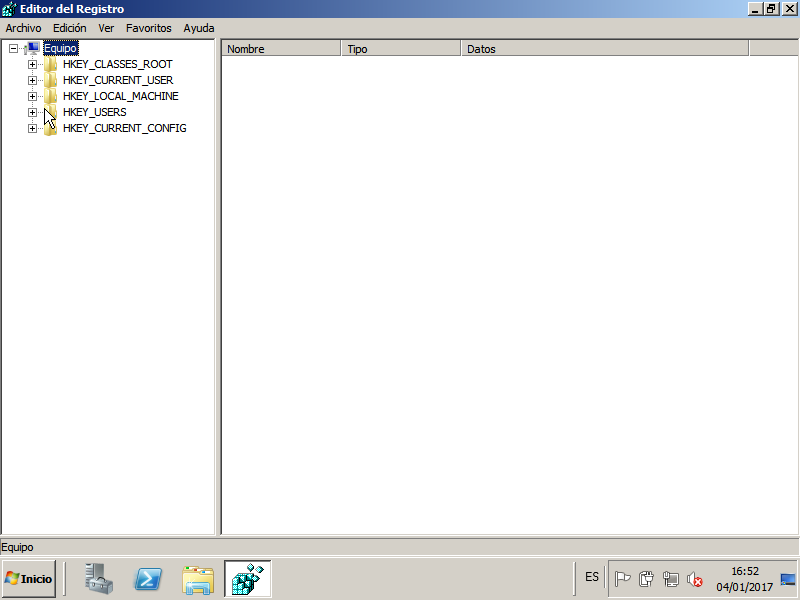
\includegraphics[scale=0.5]{imagenes/regedit2.png}  %el parámetro scale permite agrandar o achicar la imagen. En el nombre de archivo puede especificar directorios
		\caption{Pantalla inicial del editor de registro.} \label{fig:figura11}
	\end{figure}
	
	Dentro de éste podemos acceder a distintas carpetas, por ejemplo a HKEY\_LOCAL\_MACHINE que contiene los registros del sistema.
	
	\begin{figure}[H] %con el [H] le obligamos a situar aquí la figura
		\centering
		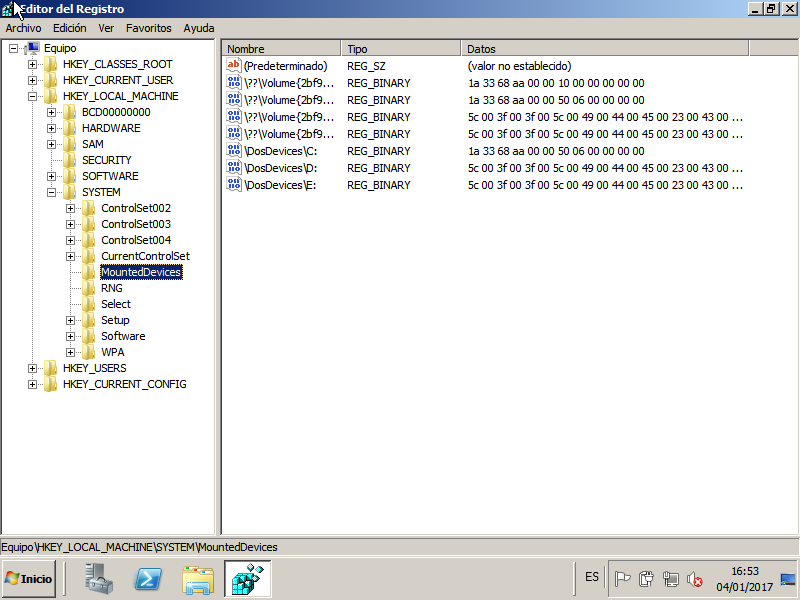
\includegraphics[scale=0.5]{imagenes/HKEY_LOCAL.png}  %el parámetro scale permite agrandar o achicar la imagen. En el nombre de archivo puede especificar directorios
		\caption{MCarpeta de registros del sistema.} \label{fig:figura12}
	\end{figure}
	
%------------------------------------------------

%----------------------------------------------------------------------------------------
%	Cuestión 4
%----------------------------------------------------------------------------------------
\section{Cuestión 4}

\subsection{\Large Enumere qué elementos se pueden configurar en Apache y en IIS para que Moodle funcione mejor.}

\begin{itemize}
	\item \Large Apache
		\begin{itemize}
			\item Ajustar el MaxClients en función de la memoria total del dispositivo, de tal forma que el máximo de clientes será el 80\% de la memoria total.
			\item Reducir el número de módulos que carga Apache en el archivo httpd.conf.
			\item Usar la última versión de Apache.
			\item Para los sistemas Unix/Linux reducir MaxRequestPerChld del archivo httpd.conf a 20-30.
			\item Establecer el parámetro "KeepAlive" a Off o bajar el valor de "KeepAliveTimeout" a un valor de 2-5, evitando así sobrecarga del procesador en el inicio de procesos.
		\end{itemize}
	
	\item \Large IIS
	
		\begin{itemize}
			\item Ajustar el valor de ListenBackLog a 2-5, que se encuentra en HKEY\_LOCAL\_MACHINE\ SYSTEM\ CurrentControlSet\ Services\ Inetinfo\ Parameters.
			\item Cambiar el valor de MemCacheSize, por defecto está al 50\% de la memoria disponible.
			\item Cambiar "MaxCachedFileSize" para ajustar el tamaño máximo de un archivo en la caché de archivos.
			\item Crear un valor DWORD llamado “ObjectCacheTTL” para cambiar la cantidad de tiempo (en milisegundos) que los objetos de la caché se mantienen en la memoria.
		\end{itemize}
\end{itemize}


No he nombrado todos elementos que se pueden cambiar en Apache para mejorar el funcionamiento de Moodle, pero se pueden encontrar todos en la página referenciada. \cite{moodle} Además, se pueden encontrar parámetros también PHP, de configuración de Hardware, etc.

%----------------------------------------------------------------------------------------
%	Cuestión 5
%----------------------------------------------------------------------------------------

\section{Cuestión 5}

\subsection{\Large 	Ajuste la compresión en el servidor y analice su comportamiento usando varios valores para el tamaño de archivo a partir del cual comprimir. Para comprobar que está comprimiendo puede usar el navegador o comandos como curl (see url) o lynx. Muestre capturas de pantalla de todo el proceso.}

El proceso para configurar la compresión del servidor viene explicado en la siguiente página. \cite{compresion}, la cual nos permite ajustar dicha compresión tanto con interfaz gráfica como por línea de comandos.

Por línea de comandos deberíamos realizar los siguientes pasos:

\begin{itemize}
	\item Para habilitar la compresión dinámica deberíamos ejecutar el siguiente comando: appcmd set config /section:urlCompression /doDynamicCompression:True
	
	\item Para habilitar la compresión estática: appcmd set config /section:urlCompression /doStaticCompression:True
	
	\item Para configurar los valores de la compresión ejecutaríamos el siguiente comando: appcmd set config /section:urlCompression /minFileSizeforComp: int /directory: string /maxDiskSpace: int


	Donde en minFileSizeforComp indicaríamos el tamaño mínimo que debe tener el archivo para ser comprimido, en directory indicaríamos dónde serán comprimidos los archivos, y en maxDiskSpace se indica el tamaño máximo de disco que podrá usar cada aplicación con la compresión estática.
\end{itemize}

En cuanto a la configuración por interfaz gráfica sería la siguiente:
Para ajustar la compresión del servidor lo que hacemos es irnos al Administrador de Internet Information Service (IIS), el cual se puede encontrar en Inicio->Todos los programas-> Herramientas administrativas-> Administrador de IIS.

\begin{figure}[H] %con el [H] le obligamos a situar aquí la figura
	\centering
	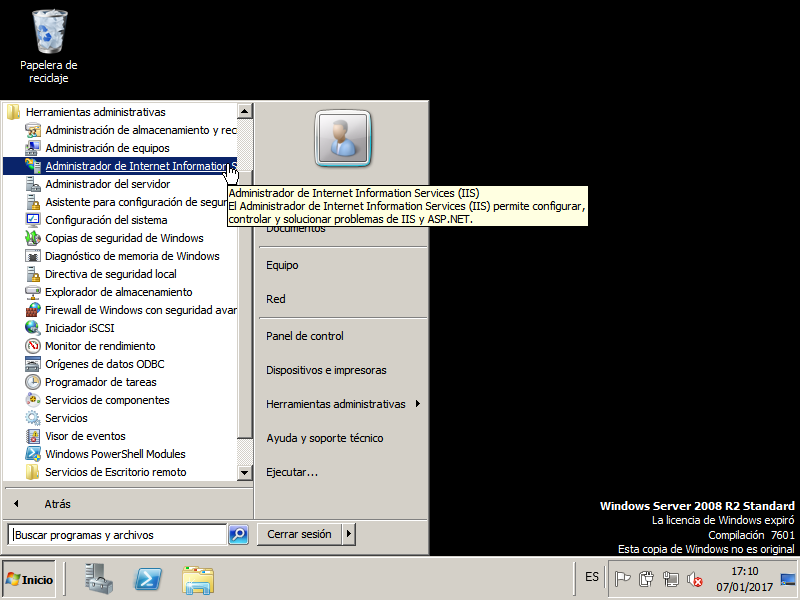
\includegraphics[scale=0.5]{imagenes/Admin_IIS.png}  %el parámetro scale permite agrandar o achicar la imagen. En el nombre de archivo puede especificar directorios
	\caption{Ruta para acceder al Administrador de IIS.} \label{fig:figura13}
\end{figure}

Una vez dentro de el Administrador, seleccionamos nuestro servidor y entre todas las opciones de administración seleccionaremos Compresión.

\begin{figure}[H] %con el [H] le obligamos a situar aquí la figura
	\centering
	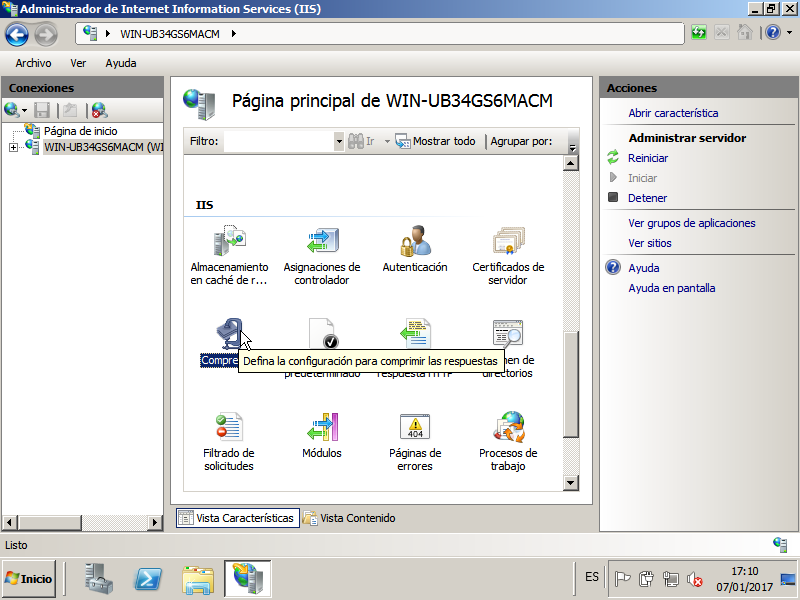
\includegraphics[scale=0.5]{imagenes/Compresion.png}  %el parámetro scale permite agrandar o achicar la imagen. En el nombre de archivo puede especificar directorios
	\caption{Elegimos la opción de compresión.} \label{fig:figura14}
\end{figure}

Una vez dentro de compresión, habilitamos las compresiones si no estuvieran habilitadas, y dentro de la compresión estática tenemos un apartado que nos permite comprimir los archivos que superen el tamaño en bytes que nosotros indiquemos.

\begin{figure}[H] %con el [H] le obligamos a situar aquí la figura
	\centering
	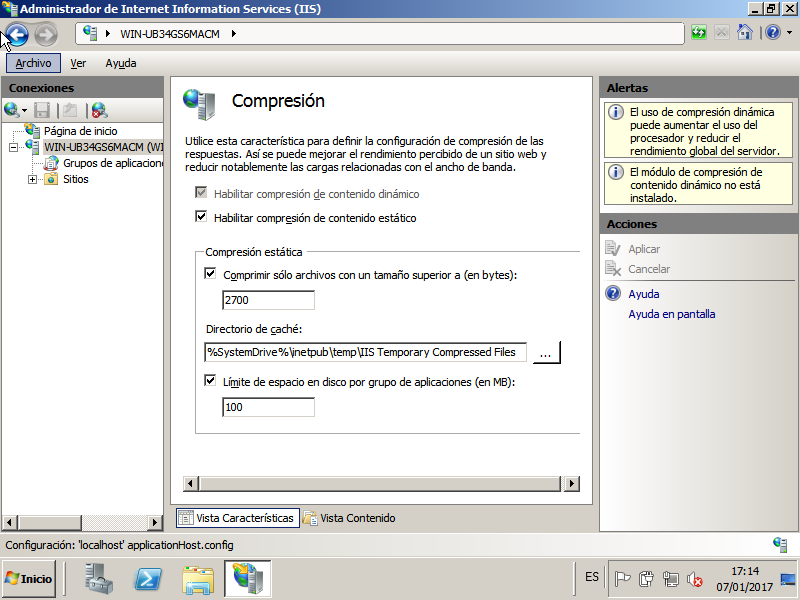
\includegraphics[scale=0.5]{imagenes/Compresion2.png}  %el parámetro scale permite agrandar o achicar la imagen. En el nombre de archivo puede especificar directorios
	\caption{Valores de nuestro primer ajuste de compresión.} \label{fig:figura15}
\end{figure}


Para comprobar que nuestro servidor comprime, vamos a entrar a firefox, iremos a la pestaña de Menú-> Desarrollador->Consola Web

Una vez ahí, nos vamos a la pestaña de Network y cargamos la página que queremos comprobar.
En las cabeceras vemos que una de ellas es Accept-Encoding la cual significa que nuestro servidor es capaz de comprimir. \cite{mozilla}

\begin{figure}[H] %con el [H] le obligamos a situar aquí la figura
	\centering
	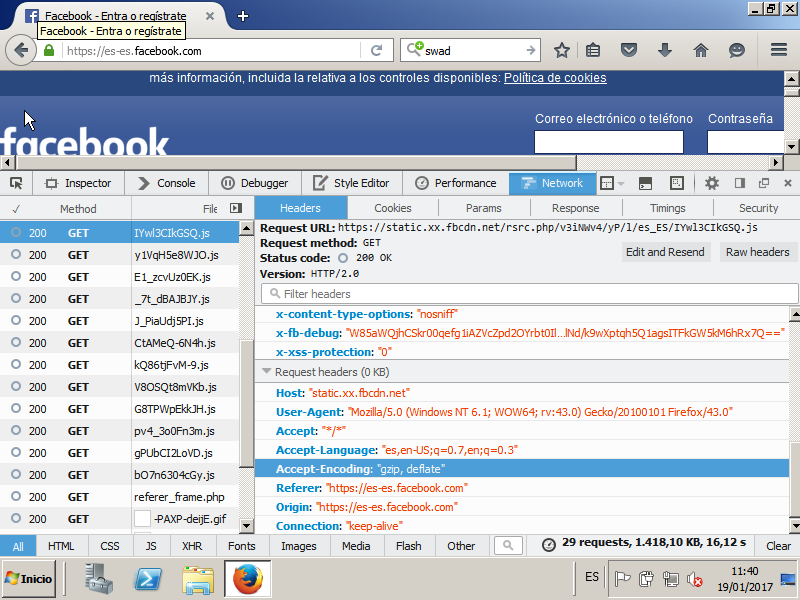
\includegraphics[scale=0.5]{imagenes/accept.png}  %el parámetro scale permite agrandar o achicar la imagen. En el nombre de archivo puede especificar directorios
	\caption{Compresión aceptada.} \label{fig:figura16}
\end{figure}



Ademas la cabecera content\_encoding nos muestra el tipo de compresión que se ha realizado, en nuestro caso gzip.
\begin{figure}[H] %con el [H] le obligamos a situar aquí la figura
	\centering
	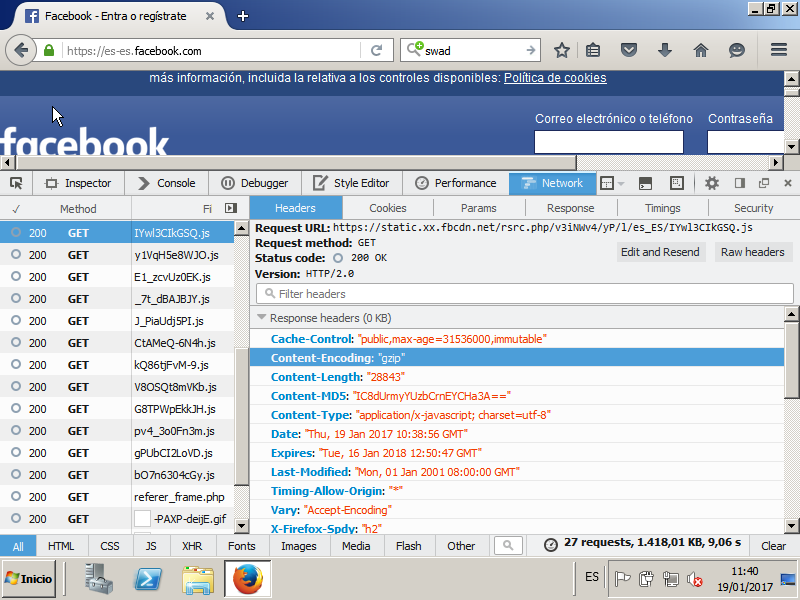
\includegraphics[scale=0.5]{imagenes/content.png}  %el parámetro scale permite agrandar o achicar la imagen. En el nombre de archivo puede especificar directorios
	\caption{Valores de nuestro primer ajuste de compresión.} \label{fig:figura17}
\end{figure}










%----------------------------------------------------------------------------------------
%	Cuestión 6
%----------------------------------------------------------------------------------------

\section{Cuestión 6}

\subsection{\Large Usted parte de un SO con ciertos parámetros definidos en la instalación (Práctica 1), ya sabe instalar servicios (Práctica 2) y cómo monitorizarlos (Práctica 3) cuando los somete a cargas (Práctica 4). Al igual que ha visto cómo se puede mejorar un servidor web (Práctica 5 Sección 3.1), elija un servicio (el que usted quiera) y modifique un parámetro para mejorar su comportamiento. Monitorice el servicio antes y después de la modificación del parámetro aplicando cargas al sistema (antes y después) mostrando los resultados de la monitorización.}

Para realizar este ejercicio vamos a usar un script realizado en Perl el cual conectará con nuestra base de datos en MySQL y nos dirá qué parámetros debemos modificar en nuestra base de datos para que mejore el rendimiento de ella.\cite{mysql}

Para ello lo primero que vamos a hacer es crear una base de datos, con una tabla a la cual le añadiremos algunos valores.
Para poder ver los tiempos de las consultas a las base de datos, primero activamos el profiler con la sentencia SET PROFILING=1 como ya hicimos en la Práctica 3.

\begin{figure}[H] %con el [H] le obligamos a situar aquí la figura
	\centering
	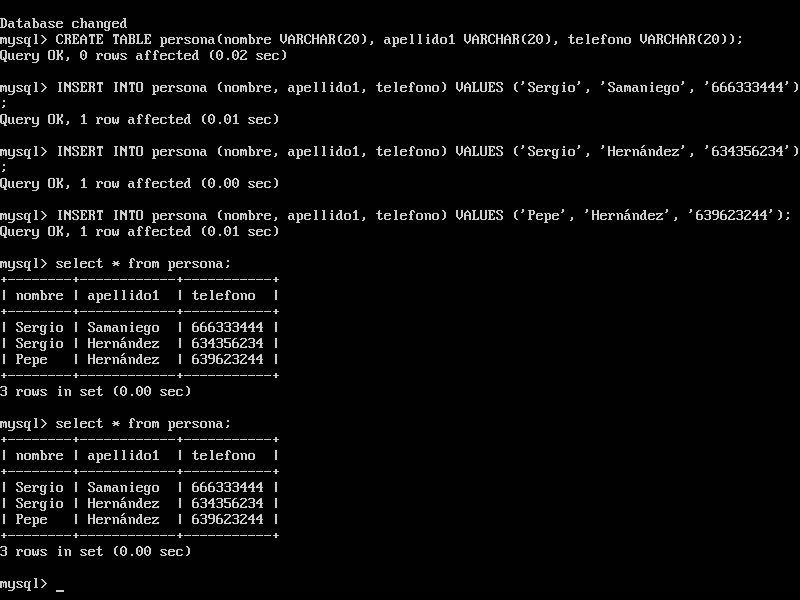
\includegraphics[scale=0.5]{imagenes/create_persona.png}  %el parámetro scale permite agrandar o achicar la imagen. En el nombre de archivo puede especificar directorios
	\caption{Creación de la tabla y de la inserción de tuplas.} \label{fig:figura18}
\end{figure}

Como vemos, si hacemos ahora SHOW PROFILES; nos mostrará los tiempos de cada una de las consultas.

\begin{figure}[H] %con el [H] le obligamos a situar aquí la figura
	\centering
	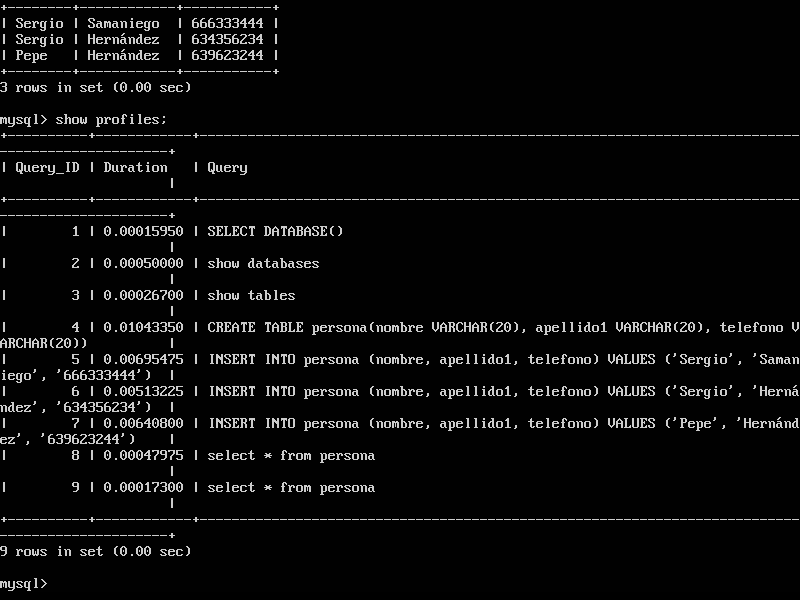
\includegraphics[scale=0.5]{imagenes/profiles1.png}  %el parámetro scale permite agrandar o achicar la imagen. En el nombre de archivo puede especificar directorios
	\caption{Tiempos de cada consulta.} \label{fig:figura19}
\end{figure}

Una vez creada la tabla, vamos a pasar el script de mysqltuner el cual hemos instalado previamente como se indica en la página referenciada,\cite{mysql} y nos dirá qué parámetros podemos cambiar en la base de datos para que mejore el rendimiento.

\begin{figure}[H] %con el [H] le obligamos a situar aquí la figura
	\centering
	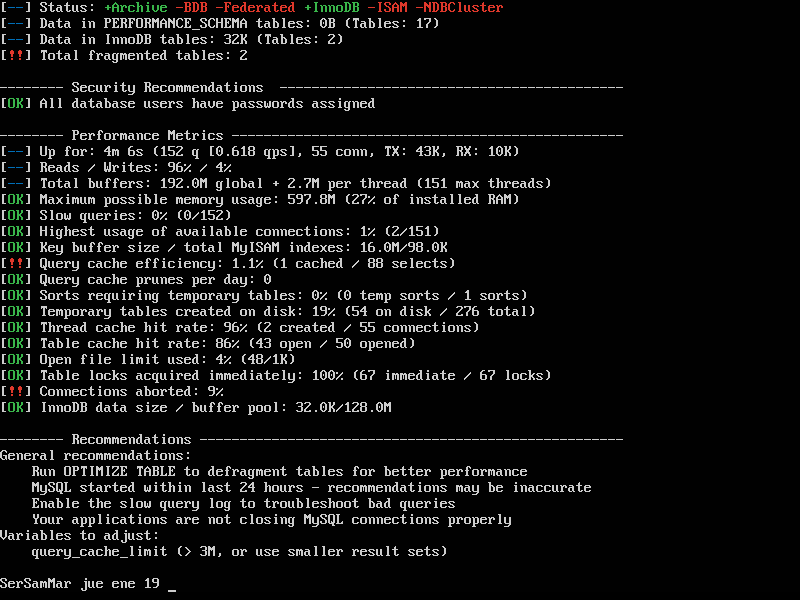
\includegraphics[scale=0.5]{imagenes/mysqltuner.png}  %el parámetro scale permite agrandar o achicar la imagen. En el nombre de archivo puede especificar directorios
	\caption{Mejoras a realizar.} \label{fig:figura20}
\end{figure}

Como vemos en la imagen, los valores que podemos modificar son :

\begin{itemize}
	\item Query\_cache\_limit: Con el cual podemos establecer el límite de caché que tendrá cada consulta.

\end{itemize}

Para poder realizar dichos cambios simplemente debemos entrar al archivo de configuración de MYSQL, que se encuentra en /etc/mysql/my.cnf 


\begin{figure}[H] %con el [H] le obligamos a situar aquí la figura
	\centering
	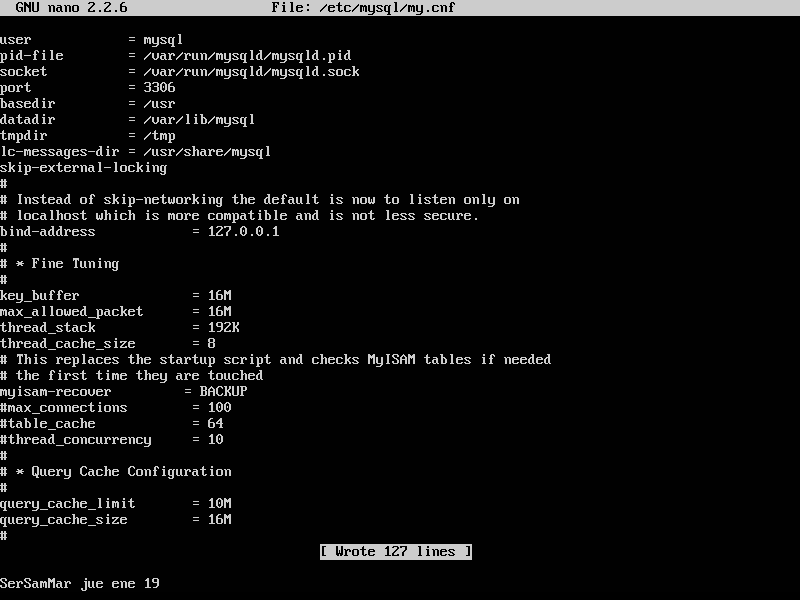
\includegraphics[scale=0.5]{imagenes/edicion.png}  %el parámetro scale permite agrandar o achicar la imagen. En el nombre de archivo puede especificar directorios
	\caption{Cambio de tamaño de Query cache limit.} \label{fig:figura21}
\end{figure}

Una vez cambiado, vamos a mirar si los resultados mejoran.
Para ello volvemos a crear una nueva tabla, con su inserción de datos, y por último veremos los tiempos de cada consulta.

\begin{figure}[H] %con el [H] le obligamos a situar aquí la figura
	\centering
	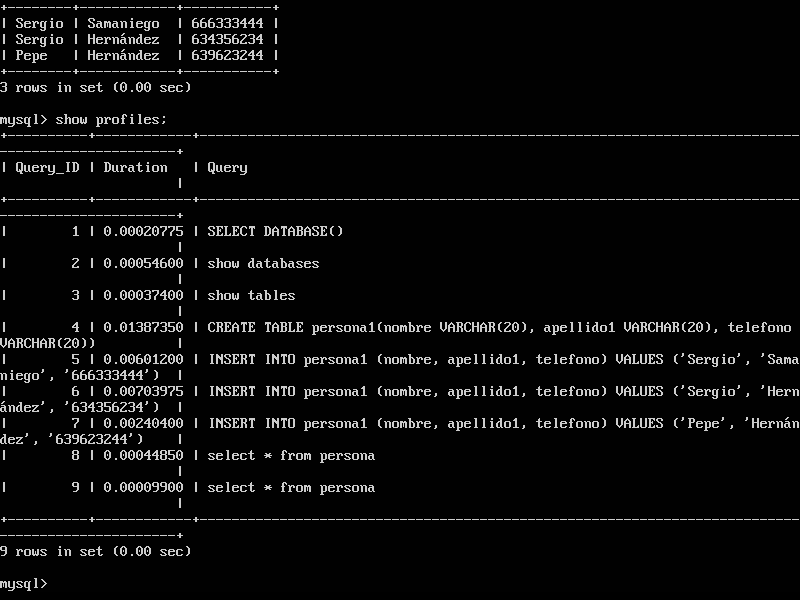
\includegraphics[scale=0.5]{imagenes/profiles2.png}  %el parámetro scale permite agrandar o achicar la imagen. En el nombre de archivo puede especificar directorios
	\caption{Tiempos con la mejora hecha.} \label{fig:figura22}
\end{figure}


Como podemos observar, la mejora de rendimiento la podemos ver en la segunda consulta de select, ya que al aumentarle el tamaño de la caché, dicha consulta se realiza más rápido que la primera, puesto que puede almacenar todo el contenido en caché.



\newpage
%------------------------------------------------

\bibliography{citas} %archivo citas.bib que contiene las entradas 
\bibliographystyle{plain} % hay varias formas de citar

\end{document}
